\subsection{Wersja 2}

\subsubsection{Opis rozwiązania}

W drugiej wersji wykorzystywany jest grid wieloblokowy o rozmiarze\footnotemark $$\frac{\text{szerokość macierzy}}{\text{szerokość bloku}} \times \frac{\text{wysokość macierzy}}{\text{wysokość bloku}}$$\\
\footnotetext{W analizowanych przypadkach wysokość macierzy jest równa szerokości macierzy, wysokość bloku jest równa szerokości bloku.}
Każdy wątek oblicza jeden element macierzy wynikowej. Pamięć współdzielona nie jest wykorzystywana.

\lstinputlisting[caption=Mnożenie macierzy kwadratowych na GPU -- wersja 2.]{./code/matrix_multiplication_2.cpp}

\subsubsection{Teoretyczna zajętość SM}

\begin{center}
\begin{table}[H]
\centering
\resizebox{\textwidth}{!}{%
\begin{tabular}{|c|c|c|c|c|c|}
\hline
\multicolumn{2}{|c|}{\multirow{2}{*}{Kryterium}} & \multicolumn{3}{c|}{Teoretyczna wartość} & \multirow{2}{*}{Limit GPU} \\ \cline{3-5}
\multicolumn{2}{|c|}{} & 8x8 & 16x16 & 22x22 & \\ \hline
\multirow{4}{*}{Zajętość SM} & Aktywne bloki & 8 & 4 & 2 & 8 \\ \cline{2-6}
& Aktywne warpy & 16 & 32 & 32 & 32 \\ \cline{2-6}
& Aktywne wątki & 512 & 1024 & 968 & 1024 \\ \cline{2-6}
& Zajętość & 50\% & 100\% & 100\% & 100\% \\ \hline
\multirow{3}{*}{Warpy} & Wątki/Blok & 64 & 256 & 484 & 512 \\ \cline{2-6}
& Warpy/Blok & 2 & 8 & 16 & 16 \\ \cline{2-6}
& Limit bloków & 16 & \textcolor{red}{\textbf{4}} & \textcolor{red}{\textbf{2}} & 8 \\ \hline
\multirow{3}{*}{Rejestry} & Rejestry/Wątek & 10 & 10 & 10 & 128 \\ \cline{2-6}
& Rejestry/Blok & 1024 & 2560 & 5120 & 16384 \\ \cline{2-6}
& Limit bloków & 16 & 6 & 3 & 8 \\ \hline
Pamięć & Pamięć współdzielona/Blok & 44 & 44 & 44 & 16384 \\ \cline{2-6}
współdzielona & Limit bloków & 32 & 32 & 32 & 8 \\ \hline
\end{tabular}
}
\caption{Teoretyczna zajętość SM -- wersja 2.}
\end{table}
\end{center}

Dla bloku 8x8 limitem okazuje się być maksymalna ilość bloków na SM, stąd zajętość $ 16 / 32 = 50\% $. \\
Dla macierzy 16x16 i 22x22 limitem są warpy. Przypada odpowiednio $ 8 $ i $ 16 $ warpów na blok, co daje limit $ 4 $ i $ 2 $ aktywnych bloków. Zajętość dla obu tych wielkości bloków ponownie wynosi $ 100\% $.

\subsubsection{Wyniki pomiarów}

\paragraph{Czas trwania obliczeń}

\begin{figure}[H]

  \begin{minipage}[c]{0.46\textwidth}
  \centering
  \resizebox{\textwidth}{!}{%
  \begin{tabular}{|c|c|c|c|}
  \hline
  Rozmiar & \multicolumn{3}{c|}{Rozmiar bloku} \\ \cline{2-4}
  macierzy & 8x8 & 16x16 & 22x22 \\ \hline
  176x176 & 1.466 & 1.381 & 2.552 \\ \hline
  352x352 & 12.934 & 11.713 & 21.462 \\ \hline
  528x528 & 38.574 & 36.721 & 66.967 \\ \hline
  \end{tabular}
  \captionlistentry[table]{Czas obliczeń [ms] -- wersja 2.}
  }

  \end{minipage}
  \qquad
  \begin{minipage}[c]{0.46\textwidth}
  \centering

  \resizebox{\textwidth}{!}{%
    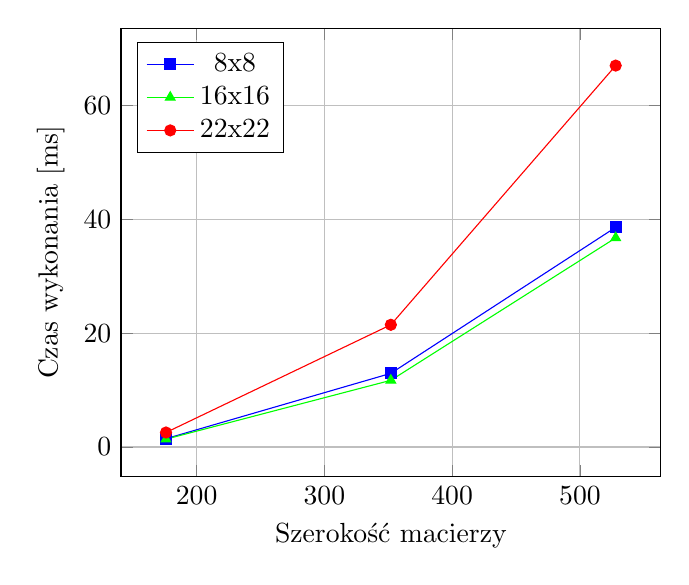
\begin{tikzpicture}
      \begin{axis}[
        xlabel=Szerokość macierzy,
        ylabel={Czas wykonania [ms]},
        legend pos=north west,
        grid=both
      ]

      \addplot[color=blue,mark=square*] coordinates {%
        (176, 1.466)
        (352, 12.934)
        (528, 38.574)
      };
      \addlegendentry{8x8}

      \addplot[color=green,mark=triangle*] coordinates {%
        (176, 1.381)
        (352, 11.713)
        (528, 36.721)
      };
      \addlegendentry{16x16}

      \addplot[color=red,mark=*] coordinates {%
        (176, 2.552)
        (352, 21.462)
        (528, 66.967)
      };
      \addlegendentry{22x22}

      \end{axis}%
    \end{tikzpicture}%
  }
  \end{minipage}

  \captionsetup{labelformat=andtable}
  \caption{Zależność pomiędzy czasem obliczeń a rozmiarem macierzy -- wersja 2.}
\end{figure}

\paragraph{Ilość operacji zmiennoprzecinkowych na sekundę}

\begin{figure}[H]

  \begin{minipage}[c]{0.46\textwidth}
  \centering
  \resizebox{\textwidth}{!}{%
  \begin{tabular}{|c|c|c|c|}
  \hline
  Rozmiar & \multicolumn{3}{c|}{Rozmiar bloku} \\ \cline{2-4}
  macierzy & 8x8 & 16x16 & 22x22 \\ \hline
  176x176 & 7.440 & 7.897 & 4.273 \\ \hline
  352x352 & 6.744 & 7.447 & 4.064 \\ \hline
  528x528 & 7.632 & 8.017 & 4.396 \\ \hline
  \end{tabular}
  \captionlistentry[table]{Ilosc operacji zmiennoprzecinkowych na sekundę (GFLOPS) -- wersja 2.}
  }

  \end{minipage}
  \qquad
  \begin{minipage}[c]{0.46\textwidth}
  \centering

  \resizebox{\textwidth}{!}{%
    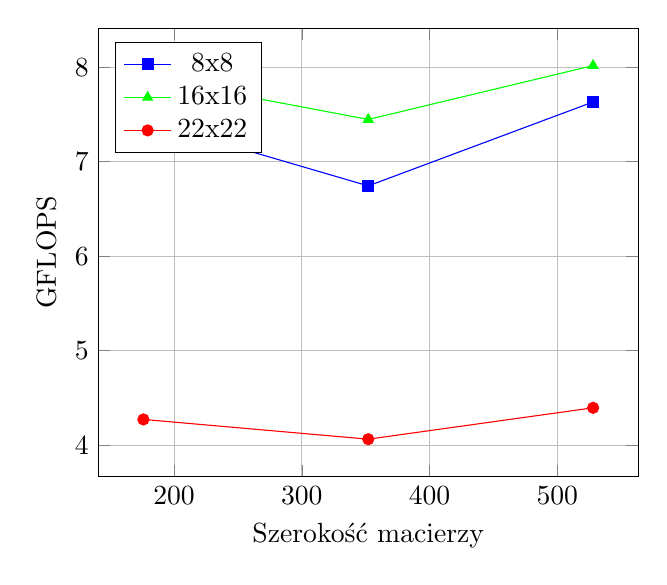
\begin{tikzpicture}
      \begin{axis}[
        xlabel=Szerokość macierzy,ylabel={GFLOPS},legend pos= north west,grid=both]

      \addplot[color=blue,mark=square*] coordinates {%
        (176, 7.440)
        (352, 6.744)
        (528, 7.632)
      };
      \addlegendentry{8x8}

      \addplot[color=green,mark=triangle*] coordinates {%
        (176, 7.897)
        (352, 7.447)
        (528, 8.017)
      };
      \addlegendentry{16x16}

      \addplot[color=red,mark=*] coordinates {%
        (176, 4.273)
        (352, 4.064)
        (528, 4.396)
      };
      \addlegendentry{22x22}

      \end{axis}%
    \end{tikzpicture}%
  }

  \end{minipage}

  \captionsetup{labelformat=andtable}
  \caption{Zależność pomiędzy ilością operacji zmiennoprzecinkowychna sekundę a rozmiarem macierzy -- wersja 2.}
\end{figure}

\paragraph{Ilość instrukcji wykonanych na sekundę}

\begin{figure}[H]

  \begin{minipage}[c]{0.46\textwidth}
  \centering
  \resizebox{\textwidth}{!}{%
  \begin{tabular}{|c|c|c|c|}
  \hline
  Rozmiar & \multicolumn{3}{c|}{Rozmiar bloku} \\ \cline{2-4}
  macierzy & 8x8 & 16x16 & 22x22 \\ \hline
  176x176 & 0.07851 & 0.08334 & 0.04509 \\ \hline
  352x352 & 0.07085 & 0.07776 & 0.04455 \\ \hline
  528x528 & 0.08095 & 0.08248 & 0.04777 \\ \hline
  \end{tabular}
  \captionlistentry[table]{Ilość instrukcji wykonana na sekundę (GIPS) -- wersja 2.}
}

  \end{minipage}
  \qquad
  \begin{minipage}[c]{0.46\textwidth}
  \centering

  \resizebox{\textwidth}{!}{%
  \centering
    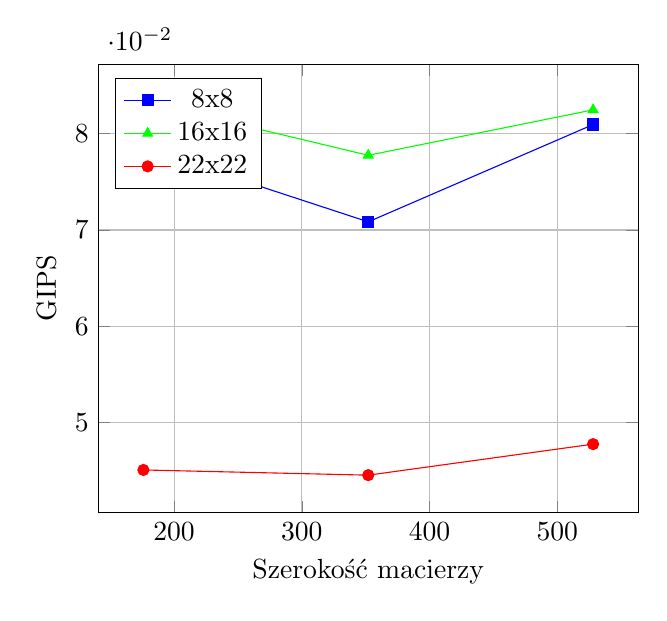
\begin{tikzpicture}
      \begin{axis}[
        xlabel=Szerokość macierzy,ylabel={GIPS},legend pos= north west,grid=both]

      \addplot[color=blue,mark=square*] coordinates {%
        (176, 0.07851)
        (352, 0.07085)
        (528, 0.08095)
      };
      \addlegendentry{8x8}

      \addplot[color=green,mark=triangle*] coordinates {%
        (176, 0.08334)
        (352, 0.07776)
        (528, 0.08248)
      };
      \addlegendentry{16x16}

      \addplot[color=red,mark=*] coordinates {%
        (176, 0.04509)
        (352, 0.04455)
        (528, 0.04777)
      };
      \addlegendentry{22x22}

      \end{axis}%
    \end{tikzpicture}%
  }

  \end{minipage}
  
  \captionsetup{labelformat=andtable}
  \caption{Zależność pomiędzy ilością instrukcji wykonanych na sekundę a rozmiarem macierzy -- wersja 2.}
\end{figure}

\paragraph{CGMA}

\begin{figure}[H]

  \begin{minipage}[c]{0.46\textwidth}
  \centering
  \resizebox{\textwidth}{!}{%
  \begin{tabular}{|c|c|c|c|}
  \hline
  Rozmiar & \multicolumn{3}{c|}{Rozmiar bloku} \\ \cline{2-4}
  macierzy & 8x8 & 16x16 & 22x22 \\ \hline
  176x176 & 21.511 & 35.852 & 23.178 \\ \hline
  352x352 & 21.422 & 32.538 & 21.322 \\ \hline
  528x528 & 21.178 & 32.267 & 21.768 \\ \hline
  \end{tabular}
  \captionlistentry[table]{Stosunek ilości operacji zmiennoprzecinkowych do ilości operacji odczytu/zapisu z pamięci globalnej -- wersja 2.}
  }

  \end{minipage}
  \qquad
  \begin{minipage}[c]{0.46\textwidth}
  \centering

  \resizebox{\textwidth}{!}{%
  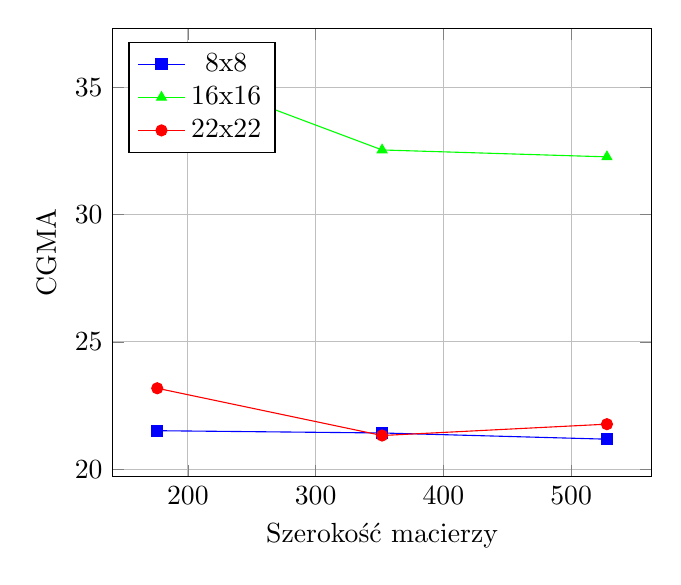
\begin{tikzpicture}
    \begin{axis}[
      xlabel=Szerokość macierzy,ylabel={CGMA},legend pos= north west,grid=both]

    \addplot[color=blue,mark=square*] coordinates {%
      (176, 21.511)
      (352, 21.422)
      (528, 21.178)
    };
    \addlegendentry{8x8}

    \addplot[color=green,mark=triangle*] coordinates {%
      (176, 35.852)
      (352, 32.538)
      (528, 32.267)
    };
    \addlegendentry{16x16}

    \addplot[color=red,mark=*] coordinates {%
      (176, 23.178)
      (352, 21.322)
      (528, 21.768)
    };
    \addlegendentry{22x22}

    \end{axis}%
  \end{tikzpicture}%
  }
  \end{minipage}

  \captionsetup{labelformat=andtable}
  \caption{Zależność CGMA od rozmiaru macierzy -- wersja 2.}
\end{figure}
